\documentclass[12pt,a4paper]{article}
\usepackage{fontawesome5}
\providecommand{\faPencilAlt}{\faIcon{pencil-alt}}
\usepackage{styles/couleurs}
\usepackage{styles/mise_en_page}
\usepackage{styles/boites}
\usepackage{styles/maths}
\usepackage{styles/figures}
\usepackage{enumitem}
\usepackage{array}
\usepackage{tabularx}
\usepackage{amsmath}
\usepackage{amssymb}
\usepackage{tikz}
\usepackage{xparse}
\usetikzlibrary{calc,patterns,arrows.meta}
\setlist[itemize]{leftmargin=1.4em,itemsep=0.15em,topsep=0.2em}
\setlist[enumerate]{leftmargin=*,itemsep=0.25em,topsep=0.25em}
\newcommand{\lignepointillee}{\noindent\dotfill\par\vspace{0.45em}}
\newcommand{\lignesreponse}[1]{%
\begin{tcolorbox}[enhanced,colback=white,colframe=NeutreC!40,boxrule=0.5pt,
arc=1.5mm,left=3mm,right=3mm,top=2mm,bottom=1mm,before skip=2pt,after skip=2pt]
\foreach \i in {1,...,#1}{\lignepointillee}
\end{tcolorbox}}
\newcommand{\titreseq}[1]{%
\begin{center}
{\sffamily\large\bfseries\color{SavoirC}#1}
\end{center}}
\begin{document}

\titreseq{Activité 1 -- Combien de segments pour une bande de carrés ?}

On accole des carrés de même taille. Deux carrés voisins partagent un côté.

\begin{center}
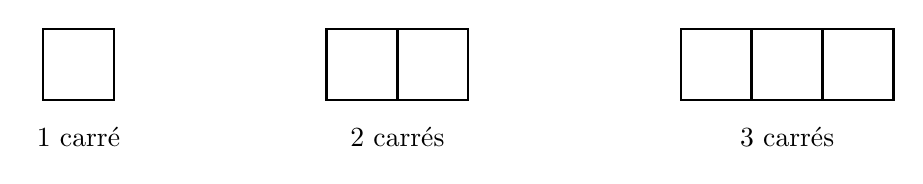
\begin{tikzpicture}[scale=0.9]
  \foreach \k/\n in {0/1,4/2,9/3}{
    \foreach \i in {0,...,\n}{
      \ifnum\i<\n
        \draw[line width=0.9pt] (\k+\i,0) rectangle ++(1,1);
      \fi
    }
    \node[below] at (\k+0.5*\n,-0.25) {\(\n\) carré\ifnum\n>1 s\fi};
  }
\end{tikzpicture}
\end{center}

\section*{Partie A -- Compter}

\renewcommand{\arraystretch}{1.55}
\begin{tabularx}{0.85\textwidth}{|>{\centering\arraybackslash}X|>{\centering\arraybackslash}X|}
\hline
\textbf{Nombre de carrés} & \textbf{Nombre de segments visibles}\\
\hline
\(1\) & \\
\hline
\(2\) & \\
\hline
\(3\) & \\
\hline
\(4\) & \\
\hline
\(10\) & \\
\hline
\end{tabularx}

\section*{Partie B -- Calculer stratégiquement}

Combien de segments sont visibles lorsqu'il y a 236 carrés?

\lignesreponse{6}

\section*{Partie C -- Décrire une stratégie}

Explique ta statégie.

\lignesreponse{6}

\newpage

\section*{Partie D -- Comparer les stratégies}

Les propositions des groupes :

\noindent
\begin{minipage}[t]{0.31\linewidth}
\begin{tcolorbox}[colback=SavoirBg, colframe=SavoirC, boxrule=0.6pt, arc=2mm]
\end{tcolorbox}
\end{minipage}\hfill
\begin{minipage}[t]{0.31\linewidth}
\begin{tcolorbox}[colback=ActionBg, colframe=ActionC, boxrule=0.6pt, arc=2mm]
\end{tcolorbox}
\end{minipage}\hfill
\begin{minipage}[t]{0.31\linewidth}
\begin{tcolorbox}[colback=NeutreBg, colframe=NeutreC, boxrule=0.6pt, arc=2mm]
\end{tcolorbox}
\end{minipage}

\noindent
\begin{minipage}[t]{0.31\linewidth}
\begin{tcolorbox}[colback=ActionBg, colframe=ActionC, boxrule=0.6pt, arc=2mm]
\end{tcolorbox}
\end{minipage}\hfill
\begin{minipage}[t]{0.31\linewidth}
\begin{tcolorbox}[colback=NeutreBg, colframe=NeutreC, boxrule=0.6pt, arc=2mm]
\end{tcolorbox}
\end{minipage}\hfill
\begin{minipage}[t]{0.31\linewidth}
\begin{tcolorbox}[colback=SavoirBg, colframe=SavoirC, boxrule=0.6pt, arc=2mm]
\end{tcolorbox}
\end{minipage}


\begin{enumerate}
  \item Explique la stratégie correspondant à chaque formule.
  \item Vérifie qu'elles donnent le même résultat pour 5 carrés.
  \item Cette vérification suffit-elle à prouver qu'elles sont toujours égales ?
\end{enumerate}

\lignesreponse{7}

\end{document}
